
The generative model, described above, is extremely data efficient at the learning phase, and generates a ranked list of 1000 grasps on a new object within 15 seconds on a 2x Intel Xeon E5-2650 v2 Eight Core 2.6GHz. There is, however, no estimate of how probable the grasp is to succeed. This the purpose of the evaluative model. Deep networks have been shown to learn good evaluative models of grasp success for two finger grippers and for dexterous hands (Barrett, Allegro) when performing what may broadly be classified as power grasps.  
%In this section, our evaluative deep network architecture is described. In the following section, the simulation used to generate the training data is detailed.
%First, the generative model largely ignores global information about the object; relying instead on global information about the hand shape, and local information about finger-object contacts. To predict grasp success probability we need a learner that somehow takes into account global information, such as global shape, mass, mass distribution, friction coefficients, deformability, etcetera. The difficulty with this is that, given a single depth image, the learner does not have direct access to these. Thus, they cannot be estimated, but all that can be learned is the association Second, the 

%It is time-consuming and expensive to collect real grasp data with using robotic arms with dexterous hands. Unlike gripper + arm combinations which require relatively less supervision \cite{Levine1}, dexterous hands can be much more fragile due to their complexity. Advances in physics simulators have made it possible to re-create robotic experiment setups in simulation. We created a simulated experimental setup in order evaluate grasp, which allowed us to collect as much data as needed in a short period of time with no supervision.
In this section, we discuss the architecture (Figure~\ref{fig:networkArchitecture}) of our evaluative network $f(I_t, h_t)$, where $I^t$ is a colorized depth image of the object, and $h_t = (h_{tw}, h_{tc})$ gives the sequence of wrist poses and hand configurations for a grasp, expressed in the camera frame used to acquire the depth image. The network outputs a grasp success probability for image-grasp pair $I_t$, $h_t$. Section~\ref{section:simulation} gives details of the simulation used to generate the training data.

% The purpose of the network is to learn the relationship between the point cloud, given as a colorized depth image, and grasp (hand shape) parameters which encode the configuration of the hand with respect to the camera frame. This is a complex task, as the kinematic model of the hand is unknown to the network, and it has to consider each grasp as a black box: The network knows the inputs that configure the hand, including the joint positions, and only has access to the outcome in the form of success/failure. 
% Talk more about the architecture
For visual processing, the network uses the VGG-16 network with weights from training on ImageNet. The final three layers are freed for training, while the first 13 layers remain frozen. Pre-processing segments the table plane from the object point cloud of the object. This segmented point cloud is then colorized. The colorization takes a 1-channel depth image $I_{t}^{depth}$ and produces a 3-channel image $I_t$ to be given as input to the VGG-16 network. First, the $640 \times 480$ depth image is cropped into a square window of size $460 \times 460$, located in the center of the image. Then, it is down-sampled to $224 \times 224$. The colorization process creates a $224 \times 224$ 3-channel image, where the first two channels of the output image $I_t$ are the mean curvature and Gaussian curvature, respectively. The third channel is the depth. %The formula of mean curvature is $h = {gr}_{xx} + {gr}_{yy}$, where ${gr}_{xx}$ is the second gradient in horizontal direction in a $1 \times 3$ window, and ${gr}_{yy}$ is its vertical counterpart. Similarly, Gaussian curvature $k = {gr}_{xx} \times {gr}_{yy} - ({gr}_{xy})^2$.
The hand trajectory $h_t$ comprises 10 way-points, each of 28 dimensions (20 for the finger joint angles, 1 for the grasp type, and 7 for the wrist pose), giving a total of 280. This is transformed to 1024 using a single layer. This and the output of the final VGG layer are added together unit-wise. Then there four fully connected layers consisting of 1024 RELU nodes each. The output is a grasp success probability, encoded by two output nodes which give success and failure probabilities, using a softmax layer.  We use the cross entropy loss in order to train the network, as shown in Equation \ref{equation:crossentropy}.
\begin{equation}
H_{y'}(y) := - \sum_{i} ({y_i' \log(y_i) + (1-y_i') \log (1-y_i)})
\label{equation:crossentropy}
\end{equation}
where $y_i'$ is the ground truth success (1) or failure (0); $y = f(I_i, h_i)$ is the predicted grasp success of grasp trajectory $h_i$, and $I_i$ is the associated colorized depth image of grasp $h_i$.
\begin{figure}
  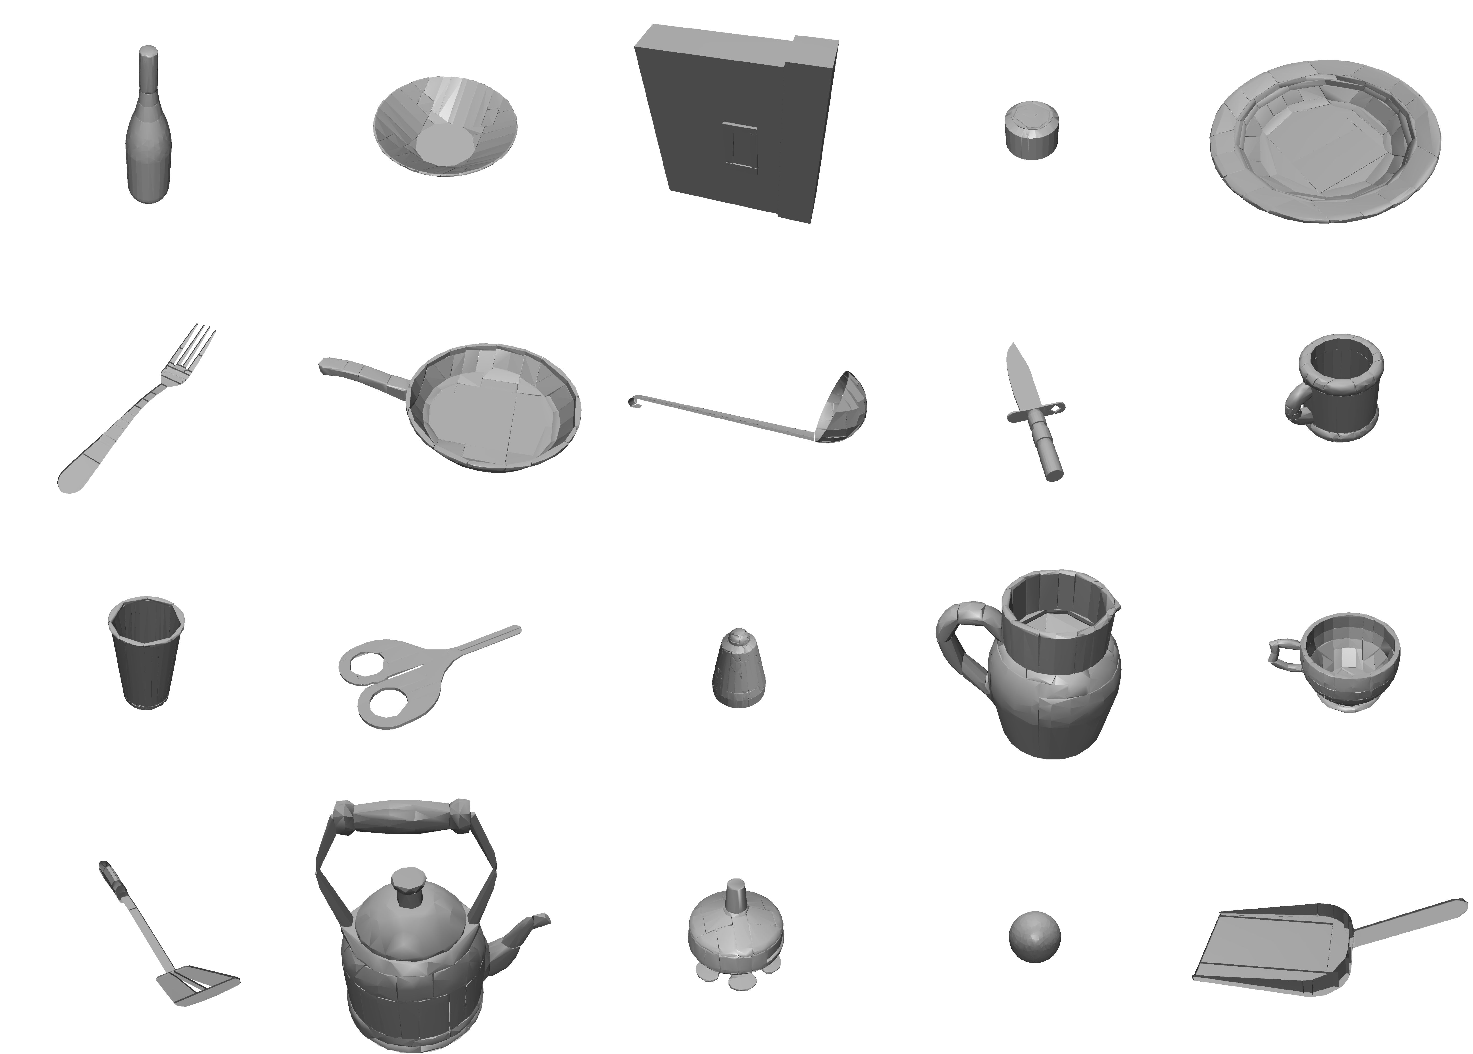
\includegraphics[width=\linewidth]{images/allObjects.pdf}
  \caption{Sample objects from all classes in the 3D model dataset.}
  \label{fig:allObjects}
\end{figure}
As described below, we trained our network on 441,312 grasps. In the next section we describe precisely the steps we took to ensure those were representative of real grasp behaviour. % o 7000 distinct scenes, where each scene contains a random instantiation of one of the objects in the dataset with varying rigid body transformations applied, as well as friction and weight changes. The network was tested on 80000 grasps on 1200 scenes of unseen objects, as well as real robot experiments, as explained in Section \ref{section:experiments}. In order to make a direct comparison with Kopicki et al. \cite{kopicki2015ijrr}, we pick top grasps based on both the original ranking, as explained in Section \ref{section:generative}, and according to the predicted success probabilities by the network. 

%We opted to use a grasp success prediction network due to the fact that the grasp generator function, explained in the previous chapter, provides alternatives of most intuitive types of grasps. A logical extension of this work would be to pair our learning algorithm with a grasp generator network, which we consider as future work.

%Overall network architecture. VGG summary. Description of new layers. Representation of hand parameters, frames of reference, camera image conversion for VGG, trajectory of wrist and fingers.